\section{Front panel}
On figure \ref{fig:front_panel}, the front panel of the crane is shown. The output row of BNC-connectors outputs the raw data from the from the sensors, the output BNC connectors are also connected to the DB-25 connector as described in section \ref{connector}. The input row of BNC-connectors are for connecting the output of an analog filter connected to the output BNC row. No data on the input BNC row is available if no connections exists between the output BNC row and the input BNC row. 

External motor drivers can be connected through the \textit{MOTOR X} and \textit{MOTOR Y} when the respective switches are flipped to \textit{DC SUPPLY}. When switched to \textit{DC SUPPLY} the ground of the relevant motors are disconnected from common ground.    

The connector \textit{POS SUP} is for supplying the potentiometer with power. This supply is also available through the DB-25 connector as Pos-supply. 

The two buttons \textit{ENABLE RESET} disconnects the \textit{ENABLE}-pins of the motor drivers for the respective axis. When pressed the \textit{ENABLE}-pins of the motor drivers are floating. 

The connector \textit{BRAKE} is not connected. 

The blue DB-25 connector shown to the left in figure \ref{fig:front_panel} gives access to both the output and input row of the front panel, which makes it possible to communicate with the digital angle sensor and to control of the motor drivers. The DB-25 connector is furthermore connected to the control inputs of the motor drivers. The pins on the DB-25 connector are listed in section \ref{connector}.

Figure \ref{fig:power_supply_panel} shows the panel for connecting external power supplies to the motor drivers. Connector \textit{EXT+} is for the positive supply. Connector \textit{SENS/EXT+} is for connecting a sense wire from the power supply. The switches switch between the internal or external power supply for the relevant motor driver, when set in neutral no power is supplied from either supplies.

\begin{figure}[H]
    \centering
    \begin{subfigure}[b]{0.47\textwidth}
        \centering
        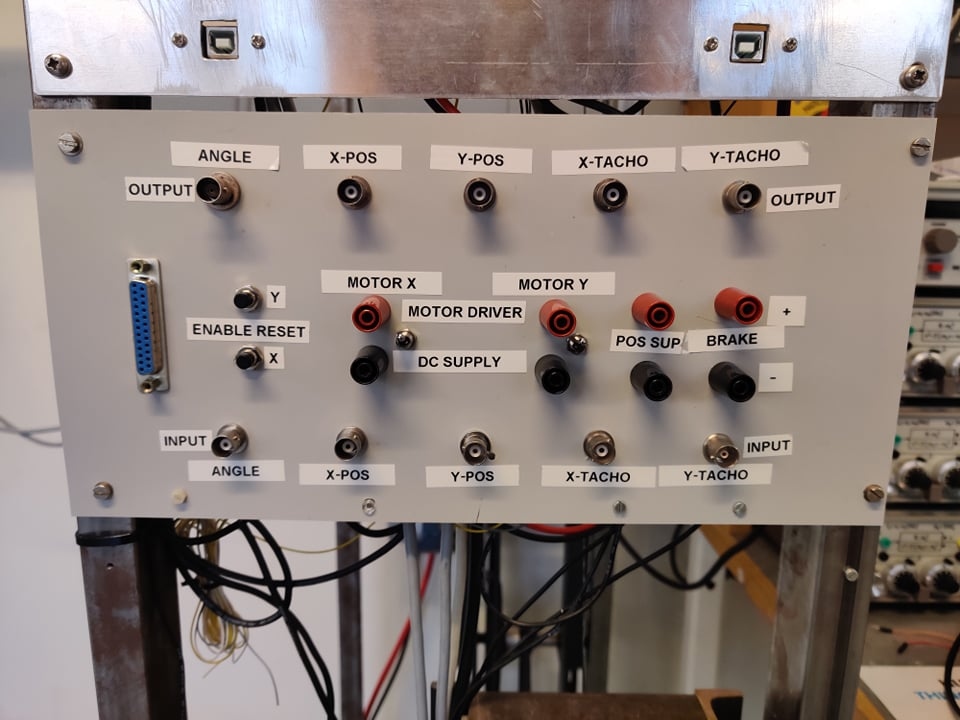
\includegraphics[width=\textwidth]{pictures/front_panel.jpg}
        \caption{The main front panel.}
        \label{fig:front_panel}
    \end{subfigure}
    \hfill
    \begin{subfigure}[b]{0.47\textwidth}
        \centering
        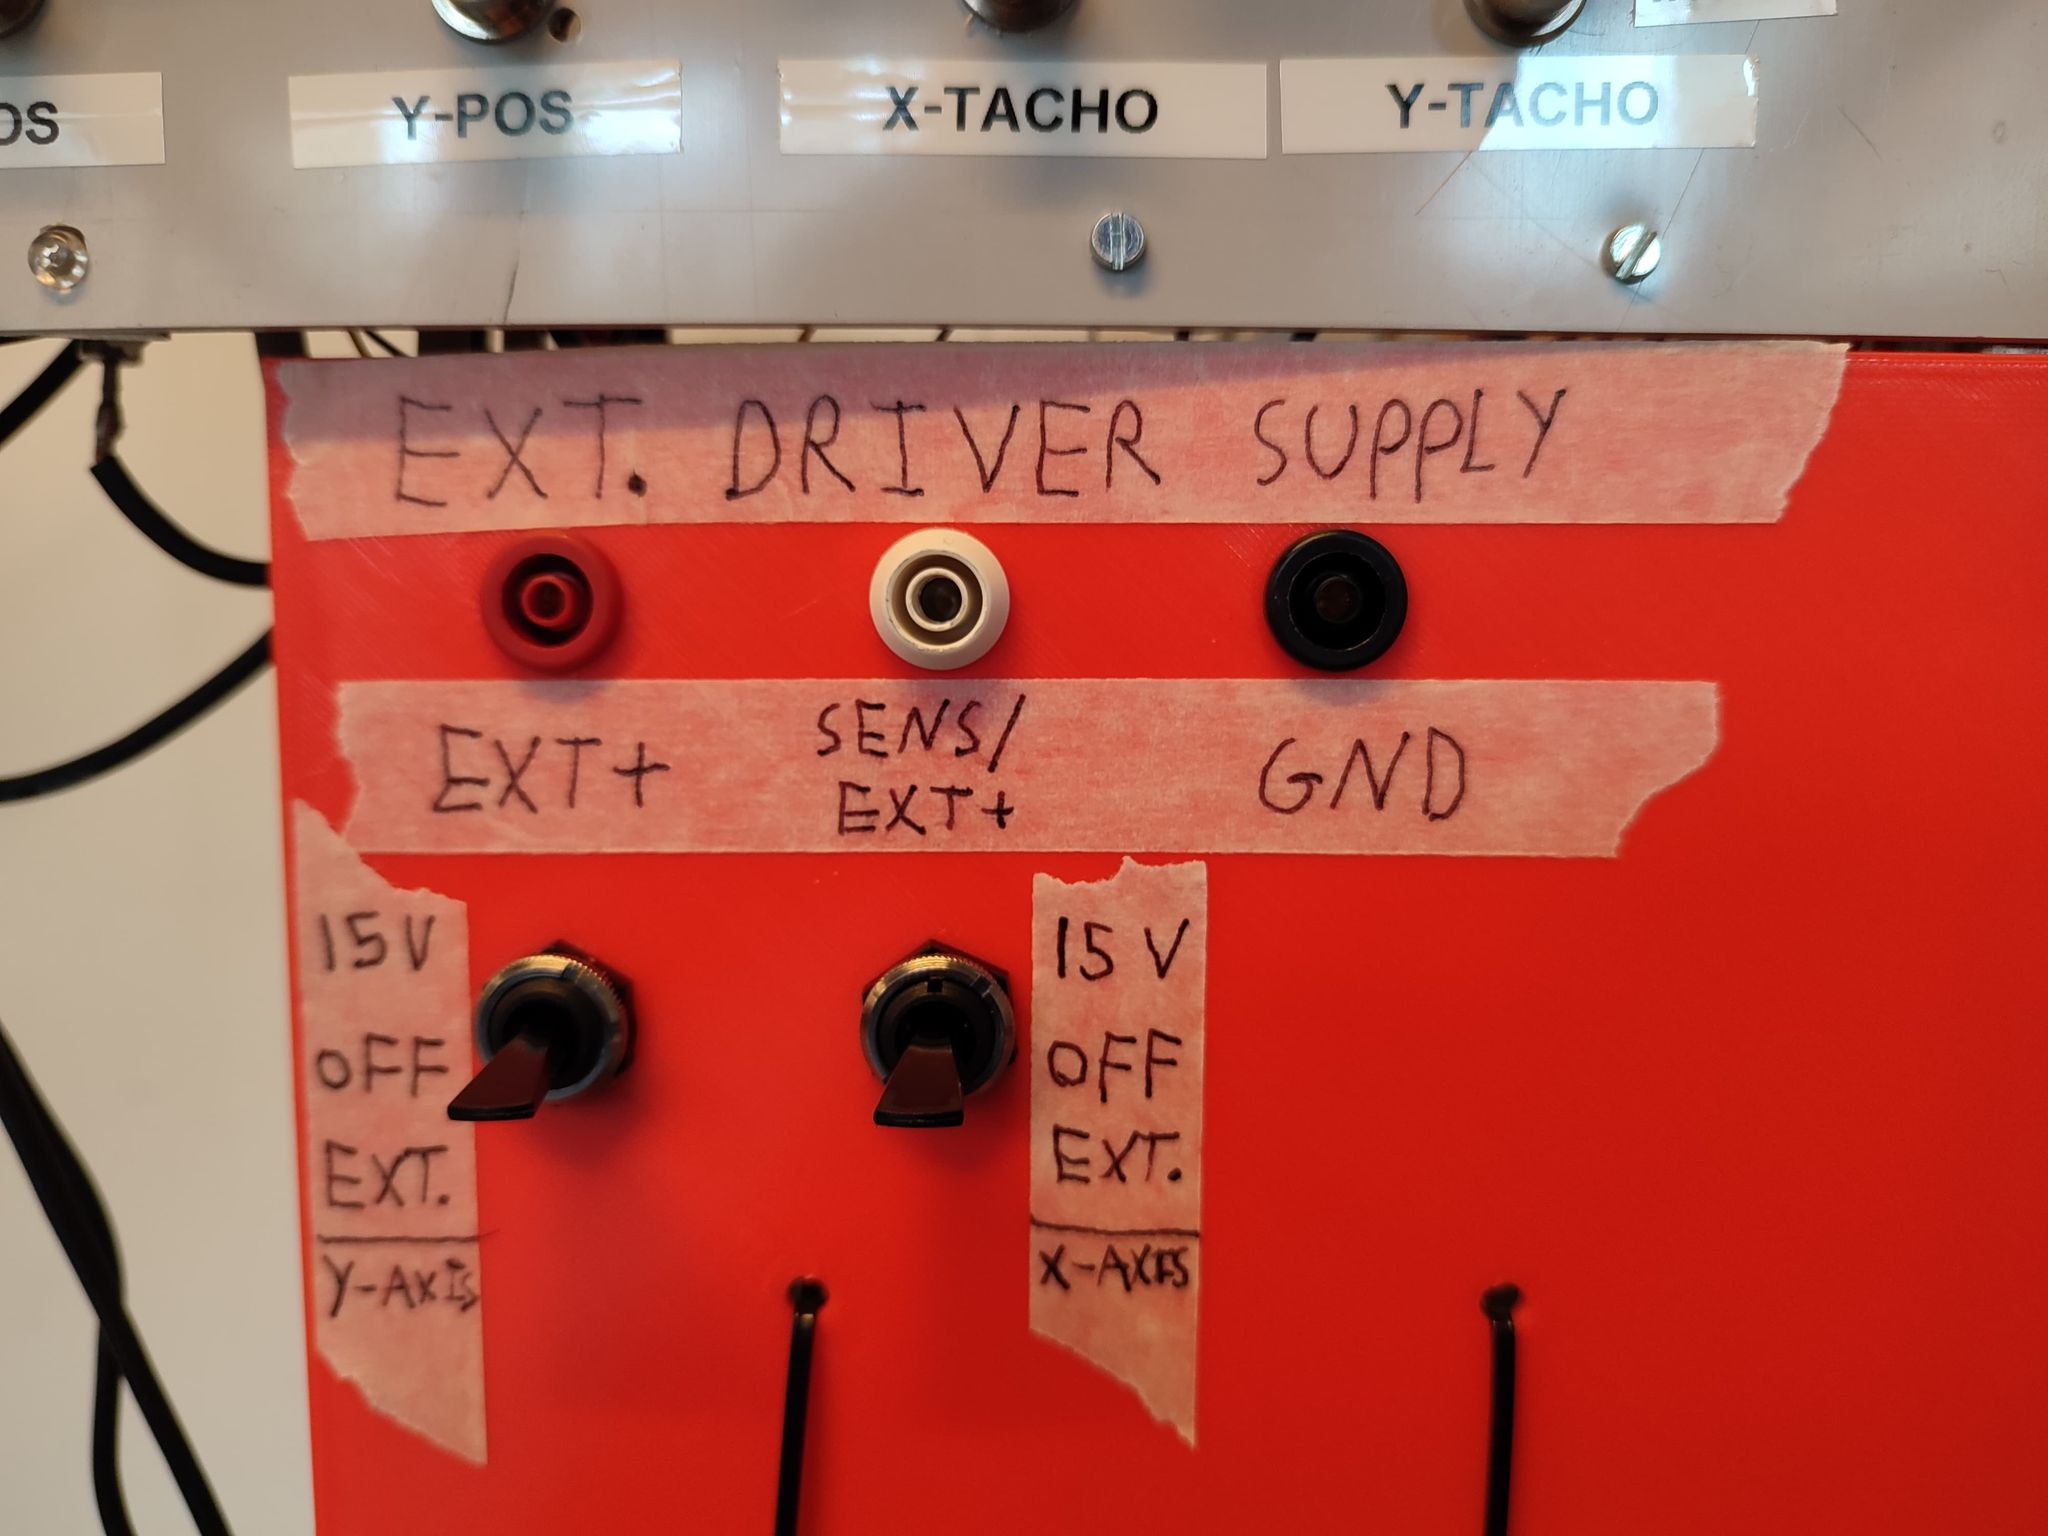
\includegraphics[width=\textwidth]{pictures/power_supply_panel.jpg}
        \caption{Panel for external supply to the motor drivers.}
        \label{fig:power_supply_panel}
    \end{subfigure}
    \caption{Figurtekst for hele figuren}
    \label{fig:crane_front}
\end{figure}


\begin{table}[H]
    \centering
    \small
    \begin{tabular}{l|l|l|l}
        \textbf{Connector} & \textbf{Category} & \textbf{Interface} & \textbf{Max ratings}\\\hline
        Angle   & Output & Digital, see section \ref{sec:angleSensor} &\SI{5}{\volt}\\ \hline
        Y-pos   & Output & Analog & \SI{5}{\volt}      \\ \hline
        X-pos   & Output & Analog & \SI{5}{\volt}      \\ \hline
        X-tacho & Output & Analog & $\pm$\SI{26}{\volt}\\ \hline
        Y-tacho & Output & Analog & $\pm$\SI{26}{\volt}\\ \hline
        Angle   & Input  & Digital, see section \ref{sec:angleSensor} &\SI{5}{\volt}\\ \hline
        Y-pos   & Input  & Analog & \SI{5}{\volt}      \\ \hline
        X-pos   & Input  & Analog & \SI{5}{\volt}      \\ \hline
        X-tacho & Input  & Analog & $\pm$\SI{26}{\volt}\\ \hline
        Y-tacho & Input  & Analog & $\pm$\SI{26}{\volt}\\ \hline
        \textit{DC SUPPLY} & Input  & Analog & \SI{11}{\ampere}\\ \hline
        \textit{POS SUP} & Input  & Analog & \SI{5}{\volt}\\ \hline
        \textit{EXT. DRIVER SUPPLY} & Input & Analog & \makecell[l]{Pulse: \SI{56}{\volt} @ \SI{15}{\ampere}\\ Cont: \SI{56}{\volt} @ \SI{5}{\ampere}}
    \end{tabular}
    \caption{Connections in the DB-25 connector, pins that are not mentioned are not connected.}
    \label{tab:DB25Pins}
\end{table}




\subsection{DB-25 connector} \label{connector}
The DB-25 connector on the front panel serves the purpose of connecting a controller to the crane with all the necessary inputs and outputs to control the crane. The connections are shown in figure \ref{fig:DB-connector} and table \ref{tab:DB25Pins}.

%https://drive.google.com/file/d/1Y5d1-83-JyrTVmY5TaLdaOAuTmAgpBFL/view?usp=sharing
\begin{figure}[]
    \centering
    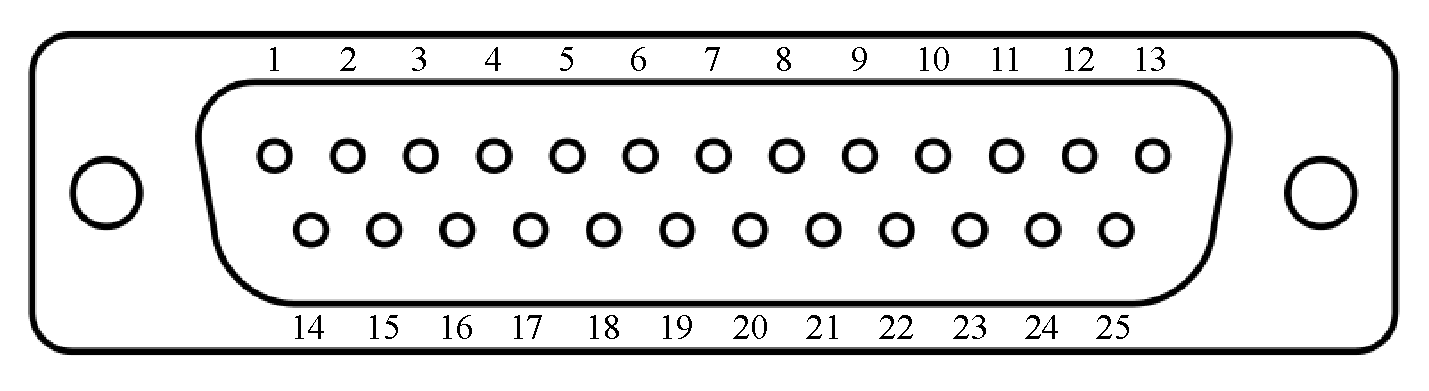
\includegraphics[width=0.6\textwidth]{pictures/DB-25 connector.pdf}
    \caption{Front panel DB-25 connector.}
    \label{fig:DB-connector}
\end{figure}

Both pin 1 and 15 are connected to the pos-supply that supply the potentiometers on the x- and y-axis with the necessary \SI{5}{V},it is only necessary to supply voltage to one of the two. Pin 3 Vin is the \SI{15}{V} supplied by the power supply mounted on the crane, this can be used to power the controller. \textbf{OBS!} All taco measurements are up to $\pm$ \SI{26}{V}, this can damage some micro controllers.

\newpage
\begin{table}[H]
    \centering
    \small
    \begin{tabular}{l|l|l|p{4.5 cm}}
        \textbf{Pin} & \textbf{Connection} & \textbf{Description} & \textbf{Interface} \\\hline
        1   & Pos-supply & Positive voltage supply from controller &STD-volt: \SI{5}{\volt}\\ \hline
        2   & Y-enable & Enables y-direction motor driver &\makecell[l]{V-range: \SIrange{0}{36}{\volt} \\ Logic 0: \SI{<1}{\volt}\\ Logic 1: \SI{>2.4}{\volt}}\\ \hline
        3   & Vin & Positive power supply to controller &STD-volt: \SI{15}{\volt}\\ \hline
        6   & Y-pos & Voltage from y-potentiometer, unfiltered & V-range: \SIrange{0}{5}{\volt}\\\hline
        7   & X-enable & Enables x-direction motor driver &\makecell[l]{V-range: \SIrange{0}{36}{\volt} \\ Logic 0: \SI{<1}{\volt}\\ Logic 1: \SI{>2.4}{\volt}}\\ \hline
        11  & Y-taco & Voltage from y-tachometer, filtered if connected &V-range: $\pm$\SI{26}{\volt}\\\hline
        12  & X-taco & Voltage from x-tachometer, filtered if connected &V-range: $\pm$\SI{26}{\volt}\\\hline
        13  & RX-head & Serial data transmitted to head & \makecell[l]{V-range: \SIrange{0}{5}{\volt} \\ Baud-rate: \SI{9600}{\baud}}\\\hline
        14  & TX-head & Serial data received from head, filtered if connected & \makecell[l]{V-range: \SIrange{0}{5}{\volt} \\ Baud-rate: \SI{9600}{\baud}}\\\hline
        15  & Pos-supply & Positive voltage supply &STD-volt: \SI{5}{\volt}\\\hline
        16  & GND & Ground connection &STD-volt: \SI{0}{\volt}\\ \hline
        17  & X-pos & Voltage from x-potentiometer, filtered if connected &V-range: \SIrange{0}{5}{\volt}\\\hline
        18  & Y-pos & Voltage from y-potentiometer, unfiltered &V-range: \SIrange{0}{5}{\volt}\\\hline
        19  & X-pos & Voltage from x-potentiometer, unfiltered &V-range: \SIrange{0}{5}{\volt}\\ \hline
        20  & Y-PWM & PWM signal for y-direction motor driver  & \makecell[l]{V-range: \SIrange{0}{36}{\volt} \\ Freq-range: \SIrange{10}{5e3}{\hertz} \\Duty-cycle: \SIrange{10}{90}{\percent}}\\ \hline
        21  & TX-head & Serial data TX, unfiltered  & \makecell[l]{V-range: \SIrange{0}{5}{\volt} \\ Baud-rate: \SI{9600}{\baud}}\\ \hline
        22  & X-PWM & PWM signal for x-direction motor driver  & \makecell[l]{V-range: \SIrange{0}{36}{\volt} \\ Freq-range: \SIrange{10}{5e3}{\hertz} \\Duty-cycle: \SIrange{10}{90}{\percent}}\\ \hline
        23  & Y-taco & Voltage from y-tachometer, unfiltered &V-range: $\pm$\SI{26}{\volt}\\\hline
        25  & X-taco & Voltage from x-tachometer, unfiltered &V-range: $\pm$\SI{26}{\volt}\\
    \end{tabular}
    \caption{Connections in the DB-25 connector, pins that are not mentioned are not connected.}
    \label{tab:DB25Pins}
\end{table}
